\documentclass[sigconf]{acmart}

%%
%% \BibTeX command to typeset BibTeX logo in the docs
\AtBeginDocument{%
  \providecommand\BibTeX{{%
    Bib\TeX}}}

%% Rights management information.  This information is sent to you
%% when you complete the rights form.  These commands have SAMPLE
%% values in them; it is your responsibility as an author to replace
%% the commands and values with those provided to you when you
%% complete the rights form.
\copyrightyear{2022}
\acmYear{2022}
\setcopyright{acmlicensed}\acmConference[MODELS '22 Companion]{ACM/IEEE 25th International Conference on Model Driven Engineering Languages and Systems}{October 23--28, 2022}{Montreal, QC, Canada}
\acmBooktitle{ACM/IEEE 25th International Conference on Model Driven Engineering Languages and Systems (MODELS '22 Companion), October 23--28, 2022, Montreal, QC, Canada}
\acmPrice{15.00}
\acmDOI{10.1145/3550356.3561540}
\acmISBN{978-1-4503-9467-3/22/10}
%%
%% For managing citations, it is recommended to use bibliography
%% files in BibTeX format.
%%
%% You can then either use BibTeX with the ACM-Reference-Format style,
%% or BibLaTeX with the acmnumeric or acmauthoryear sytles, that include
%% support for advanced citation of software artefact from the
%% biblatex-software package, also separately available on CTAN.
%%
%% Look at the sample-*-biblatex.tex files for templates showcasing
%% the biblatex styles.
%%

%%
%% The majority of ACM publications use numbered citations and
%% references.  The command \citestyle{authoryear} switches to the
%% "author year" style.
%%
%% If you are preparing content for an event
%% sponsored by ACM SIGGRAPH, you must use the "author year" style of
%% citations and references.
%% Uncommenting
%% the next command will enable that style.
%%\citestyle{acmauthoryear}

\begin{document}

%%
%% The "title" command has an optional parameter,
%% allowing the author to define a "short title" to be used in page headers.
\title{Support for OCL Libraries and Static Features}

%%
%% The "author" command and its associated commands are used to define
%% the authors and their affiliations.
%% Of note is the shared affiliation of the first two authors, and the
%% "authornote" and "authornotemark" commands
%% used to denote shared contribution to the research.
\author{Edward D. Willink}
\email{ed_at_willink.me.uk}
\affiliation{%
  \institution{Willink Transformations Ltd.}
%%  \streetaddress{P.O. Box 1212}
  \city{Reading}
  \state{Berks}
  \country{England}
%%  \postcode{43017-6221}
}

%%
%% By default, the full list of authors will be used in the page
%% headers. Often, this list is too long, and will overlap
%% other information printed in the page headers. This command allows
%% the author to define a more concise list
%% of authors' names for this purpose.
%%\renewcommand{\shortauthors}{Trovato et al.}

%%
%% The abstract is a short summary of the work to be presented in the
%% article.
\begin{abstract}
  Libraries provide a powerful re-use capability allowing developers of one application to exploit the developments of others. Sadly, OCL has no first class library capability and attempts to use available capabilities have not led to any re-usable libraries. Problems include lack of support for imports, foreign language calls, object creation, maps and inadequate specification of static features. We combine previous and new resolutions prototyped in Eclipse OCL to make libraries feasible. 
\end{abstract}

%%
%% Keywords. The author(s) should pick words that accurately describe
%% the work being presented. Separate the keywords with commas.
\keywords{OCL, Library, Native Call, Code Generation, Static Feature}

%%
%% This command processes the author and affiliation and title
%% information and builds the first part of the formatted document.
\maketitle

\section{Introduction}\label{Introduction}
Libraries provide a powerful mechanism for providing re-use. The extreme polymorphism of Java's Object and Collection classes and the consequent ease of use demonstrates how libraries can create a virtuous adoption cycle. In contrast, C++ was overtaken as its Standard Template Library arrived over ten years late and was compromised by a need to support bare arrays as collections. In further contrast, OCL has only a built-in library and few users.
  
The obvious utility of libraries has prompted authors \cite{Baar2011},\cite{Cabot2012} to query where the OCL math library is. There is no answer. In this paper, we review the inadequate support for libraries and then  provide the technology to support them. We will find that the non-Object Oriented style of typical mathematical operations requires the semantics of static features in OCL to be resolved.

OCL 2.0~\cite{OCL-2.0} attempts to formalize the intuitive obviousness of OCL 1.x with the aid of models. Unfortunately the formalization never progressed beyond the draft stage and so whenever we look too closely at OCL 2.0 we find incompleteness and inconsistency \cite{Willink2020}. The Abstract Syntax model omits critical classes such as \verb|VariableDeclaration|. There is no model of the library, just many well-intentioned partial specifications.

In \cite{Willink2011}, Eclipse OCL~\cite{Eclipse-OCL} introduced a model and grammar for the OCL Standard Library supported by an Xtext editor. The library model declares the library types and their features including template parameters.

\begin{figure}
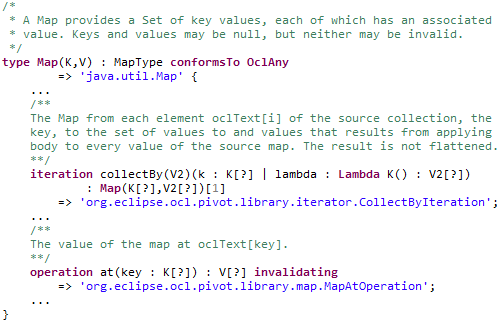
\includegraphics[width=\columnwidth]{OCLstdlib.png}
\caption{OCLstdlib model example.}
\Description{OCLstdlib model example}
\label{fig:oclstdlib}
\end{figure}

Figure~\ref{fig:oclstdlib} shows part of the declaration of the \verb|MapType| with \verb|K| and \verb|V| template parameters. An iteration with a \verb|V2| template parameter and an operation are also shown. The operation demonstrates the fairly strong modeling identifying that the templated argument and return may be null. Additionally the \verb|invalidating| keyword indicates that the result may be \verb|invalid|. The iteration declares its potentially null parameter followed by its body typed as a lambda-expression\footnote{The bodies of iterations are lambda expressions in all but name.}. The return is a non-null map of potentially null keys and values.

The figure also demonstrates using \verb|java.util.Map| for the native implementation of the type, and using a custom helper class for each operation and iteration. The helper classes use polymorphism to dispatch \verb|OperationCallExp::referredOperation| rapidly.

Once the OCL Standard Library was modeled, it was possible to separate the OCL Language from the OCL Standard Library allowing a user to provide an alternate or extended library implementation. It was also possible to define additional libraries. A few JUnit tests demonstrated the principle within Eclipse OCL, however an attempt to write a tutorial to show users how to exploit the potential of an additional library demonstrated that the implementation was not ready for prime time\footnote{https://bugs.eclipse.org/bugs/show\_bug.cgi?id=415146}.

%The tutorial was stuck on my to-do list until Kevin Lano suggested collaborating on a Masters project to provide an OCL library. Despite the funding falling through, I proceeded to investigate the library problems and long overdue solutions that are reported in this paper.

We first review the ergonomic issues to be solved in Section~\ref{Library Ergonomics} then in Section~\ref{Examples} we examine a few examples that motivate exploiting static features whose semantics we examine in Section~\ref{Static Semantics}. In Section~\ref{Status} we describe the status of this work and in Section~\ref{Further Work} we take static properties further. Then in Section~\ref{Related Work}, we look at other work, before concluding in Section~\ref{Conclusion}.
  
\section{Library Ergonomics}\label{Library Ergonomics}
 
In order to make a library useful we need to solve four problems for the user.

\begin{itemize}
	\item import the library of declarations
	\item specify the library declarations
	\item implement each library declaration
	\item invoke a specific library declaration
\end{itemize}

\subsection{Import}
 
The OCL specification~\cite{OCL-2.4} defines a language that can usefully constrain models, but does not specify where the models come from. This provides considerable flexibility but has prevented vendors from providing a general solution. Each tool has its own proprietary solution to solving the relationship between the OCL programming and the models with their metamodels.

Complete OCL comes closer to being complete in so far as the specification defines a self-standing document with a grammar that can complement a model. However a practical implementation must either add some form of import statement to allow the Complete OCL document to reference its complemented models, or operate in a pre-loaded context with ready to-go models.

A similar import statement or pre-loading will be needed to exploit a library of declarations. This should be just a variation of a proprietary facility that we do not need to address further here. Eclipse OCL supports an import such as:

\begin{verbatim}
import 'https://git.eclipse.org/r/plugins/gitiles
  /ocl/org.eclipse.ocl/+/refs/heads/master/plugins
  /org.eclipse.ocl.pivot/model/Types.ocl'
\end{verbatim} 

\subsection{Declare}

A Complete OCL document, a UML model or Eclipse OCL's Standard Library model provide adequate mechanisms for declaring many, but perhaps not all, declarations. A minimal \verb|maths.ocl| supporting just the \verb|tan| operation could be declared as\footnote{... denotes functionality that has been omitted in order to focus on a relevant issue.}:

\begin{verbatim}
  package maths
  context Real
  def: tan() : Real = ...
  endpackage
\end{verbatim} 

\subsection{Implement}

OCL is probably Turing complete, see Section~\ref{Turing Complete}, so it is in principle possible to implement any library functionality in OCL and embed that implementation as the body of a Complete OCL declaration.

However few users will be keen to transliterate existing implementations from their favorite language in order to use them within OCL. We therefore have a vicious circle whereby the lack of any OCL libraries imposes a significant barrier to development of any OCL libraries.

Even if a good algorithm for \verb|tan| is available, there may be Intellectual Property issues that prevent its re-use. The transliteration must be tested for interesting corner cases. Transliteration alone is not sufficient.

OCL needs a mechanism to enable re-use of an implementation already available in a foreign language.

\subsection{Invoke}\label{Call}  

If the imported library declarations integrate well with other OCL declarations, the existing call capabilities should be re-usable.

\begin{verbatim}
  2.5e1.tan()
\end{verbatim} 

However when we come to implement the library declaration we find that we have just moved the problem sideways; we still need a mechanism to invoke a foreign language implementation.
(And once we provide a foreign language call, we don't need a library at all.)

A generalization of an existing solution can solve this call problem too.
The existing problem arises when the surrounding OCL context fails to provide an `import' for MyPackage as in:

\begin{verbatim}
    ...oclIsKindOf(MyPackage::MyClass)
\end{verbatim} 

The existing solution exploits the \verb|_'...'| escape mechanism for identifiers with awkward characters. A URI-qualified name can be specified as:

\begin{verbatim}
    ...oclIsKindOf(
    _'http://org.my.spec/2022#MyPackage'::MyClass)
\end{verbatim} 

We can generalize this to exploit a Java String function that the OCL String type does not support as: 

\begin{verbatim}
thisString.
  _'java:java.lang.String.compareToIgnoreCase'
    (thatString)
\end{verbatim} 

The escaped name specifies a \verb|java| language scheme followed by a Java-specific \verb|java.lang.String.compareToIgnoreCase| fully qualified name.

The names are unpleasantly long, requiring multiple lines for this paper, but at least they can work for object methods with compatible types.

Once we support the invocation of arbitrary Java operations, we undermine the guarantee that OCL is side-effect free. The author of a foreign operation call is ultimately responsible for guaranteeing that the called operation is side effect free. Section~\ref{Side-effect Free} discusses enforcing the guarantee.
%, although many abuses could be detected at the cost of a comparison of %shallow hashes of before and after parameters.

\section{Examples}\label{Examples}

We have so far considered \verb|tan| as an example. We will now change to looking at the syntactically more challenging \verb|pow| before moving onto look at Complex numbers and then \verb|Employee::uniqueId()|. 

\subsection{Math.pow}

Most languages support a functional call of \verb|tan| as \verb|tan(2.5e1)| or \verb|tan 2.5e1| rather than the Object-Oriented \verb|2.5e1.tan()| which can be supported by declaring a regular \verb|Real::tan()| operation. This OO style is strange if we want \verb|pow(2, 4)| rather than \verb|2.pow(4)|.

An OO style is not actually necessary since OCL 2.2~\cite{OCL-2.2} added support for a \verb|static| keyword when declaring operations and properties.

We may therefore provide a minimal \verb|maths.ocl| as

\begin{verbatim}
  package maths
  context Real
  static def: pow(mant : Real, expt : Real) : Real
    = _'java:java.lang.Math.pow'(mant, expt)
  endpackage
\end{verbatim} 

This can support the call from regular OCL as

\begin{verbatim}
  ... maths::Real::pow(2, 4) ...
\end{verbatim} 

If the proprietary import mechanism exposes the contents of the \verb|maths| package, the \verb|maths::| qualification and perhaps even the \verb|Real::| qualifications can be omitted giving a more optimal exposition for the call.

While OCL 2.2 added the \verb|static| keyword to the grammar, it is hard to characterize the change as more than a me-too catch-up to align with UML static features. Very little run-time semantics was provided for OCL, and there is little to infer from UML~\cite{UML-2.5.1}. Section 7.5.10 of the OCL specification provides an example that we shall see in Section~\ref{UniqueId} is not fully implementable in OCL\footnote{Diligent readers of the OCL specification may find a StaticValue class that is nothing to do with the static declaration of a feature. Rather it is a confusing throwback to when UML 1.x referred to the embedded DataType-typed attribute slots of an instance as its static structure.}. Whether and how \verb|static| is supported is down to the enthusiasm of the OCL tooling implementer.

It may be noted that Ecore~\cite{Eclipse-EMF} has no support for static features, so that if a UML model with static feature is converted using UML2Ecore, the \verb|static| keyword is ignored.

Using an OO style:

\begin{verbatim}
    ... 2.pow(4) ...
\end{verbatim} 

may workaround the absence of support for static in the grammar, but the underlying Java function is static so internal support for foreign static calls is unavoidable.

For the semantics of static operations, intuitive common sense seems adequate. For static properties we need to clarify the semantics in respect of when a `new' static instance is created and initialized. See Section~\ref{Static Semantics}.

Once we have a foreign call syntax, the user has a choice. The foreign calls can be used directly avoiding any need for a library at the expense of some clumsiness in the call expressions. Alternatively the foreign calls may be hidden within a library that provides friendly declarations that delegate to the foreign call.

In practice development/prototyping may use the direct call and evolve to use the more readable library delegation.

\subsection{Complex}

The foreign call delegation for \verb|pow| can be appropriate when the types are simple and when the implementation is too complicated to re-implement.

But consider a Complex class, which strangely Java does not provide. Even if there was a Java implementation, we might choose to re-implement since Complex is rather simple. Except that we cannot, since, in general, addition of two complex numbers creates a new complex number. OCL provides no \verb|new| capability since construction of a new object creates a side effect in the memory system. This can be seen by considering how a \verb|new| capability might work:

\begin{verbatim}
new Complex{real=2,imag=3} = new Complex{real=2,imag=3}
\end{verbatim} 

Obviously two same-valued complex numbers should be equal; this is the UML DataType semantics. But if Complex is a Class, each call to \verb|new| creates a new instance; they should therefore be different in accordance with UML Class semantics. (Java provides alternative \verb|=| and \verb|equals| facilities that allows a free and confusing choice of DataType or Class semantics.)

The problem with \verb|new| was discussed at the Aachen workshop~\cite{OCL-Aachen} where the helpful term `shadow' object was coined for the solution~\cite{Willink-Shadow}.

In principle, let all possible instances of all possible classes have a permanent shadow existence, so that whenever the Tuple syntax is used to `create' an object, the appropriate shadow instance is returned avoiding the side effect. Rewriting our example:

\begin{verbatim}
Complex{real=2, imag=3} = Complex{real=2, imag=3}
\end{verbatim} 

the two creations each return the same immutable shadow object and so the equality is satisfied. 

In practice, creation of all possible instances of all possible classes will run out of time and memory long before any useful computation can be performed. Each required shadow instance must therefore be created lazily. 

This shadow object `creation' is exactly what is needed to enable a library to support the operations of a Complex type.

\begin{verbatim}
  context Complex
  def: real : Real
  def: imag : Real
  static def: new(real : Real, imag : Real) : Complex
    = Complex{ real = real, imag = imag }
  static def: add(x1 : Complex, x2 : Complex) : Complex
    = Complex{
        real = x1.real + x2.real,
        imag = x1.imag + x2.imag
      }
\end{verbatim} 

\subsection{Unique id}\label{UniqueId}

Section 7.5.10 of the OCL specification provides half an example demonstrating how the static \verb|Employee::uniqueID| operation can be used to provide a unique ID for each \verb|Employee|.
\begin{verbatim}
  context Employee::id : String
    init: Employee::uniqueID()
\end{verbatim} 

\paragraph{Lazy (Java) Solution}

\begin{verbatim}
private static int counter = 0;
public static String uniqueID() {
    return Integer.toString(counter++);
}
\end{verbatim} 

As shown above, \verb|Employee::uniqueID| can easily be realized in Java by defining a static counter for the IDs and incrementing the counter for each invocation.

An alternative eager approach in which all IDs are allocated together is awkward since it requires access to all instances that may need IDs. This includes those instances that are yet to be created.

\paragraph{Eager (OCL) Solution}

\begin{verbatim}
static context Employee::insts : Sequence(Employee)
  init: Employee::allInstances()->asSequence()
context Employee::uniqueID() : String
  init: insts->indexOf(self).toString()
context Employee::id : String
  init: Employee::uniqueID()
\end{verbatim} 

The lazy approach cannot be written in OCL since the updates to the static counter constitute a side effect that is illegal in OCL. The eager approach above is possible since \verb|allInstances()| can find the instances and since the lack of side effects guarantees that no later creation of instances can occur.

The static \verb|Employee::insts| property is initialized once with a sequence of all \verb|Employee| instances. Thereafter each access of the \verb|Employee::uniqueID()| operation is able to compute a distinctive \verb|self|-dependent value by searching for the index of \verb|self| in \verb|Employee::insts|. The derived \verb|Employee::id()| property delegates to \verb|Employee::uniqueID()| for the first access. Subsequent accesses should benefit from a cache.

It seems unreasonable that the simple efficient lazy approach cannot be written in OCL. The semantics of static OCL features is unspecified, so there are opportunities for a resolution. Perhaps the initializer for a static property should be re-evaluated for each access. Alternatively the semantics could be refined so that the \verb|init| initializes on the first access and a \verb|der| updates on subsequent accesses. This would allow the count to evolve, but an unstable static property seems deeply suspect.

It also seems unreasonable that further instances cannot be created after some unique IDs are allocated. But for pure OCL, this is not a problem since OCL has no ability to assign or mutate; the counter with its incrementing value cannot exist. Once OCL is embedded, perhaps in QVTo~\cite{QVT-1.3}, the imperative capabilities allow successive assigns and so the lazy approach can work. Alternatively when embedded in a strongly declarative context such as QVTr, all instances exist before the `atomic' transformation completes and so it is just a scheduling challenge for the tooling to assign the IDs to the output in a timely fashion that satisfies the write/read dependencies. For pragmatic OCL enriching a model, it is the modeling environment's responsibility to reset all caches before each execution of some OCL-defined functionality; \verb|allInstances()| must be `recomputed' each time the modeling environment makes a significant change to the system state. 

%To complete the OCL specification example, we just need to allocate a distinct ID to each element of an \verb|allInstances()|. We cannot do this within uniqueID since there is no ability for a first call to populate the results for other calls. The `global' \verb|allInstances()| algorithm must be computed and cached `globally' and so must use a static cache populated before OCL execution starts. The individual results are readily accessed from the static \verb|instances| cache. 

Unfortunately the \verb|indexOf()| in our solution contributes to a quadratic implementation cost. We can linearize the cost by using a Map~\cite{Willink-Map}.

\begin{verbatim}
static context Employee::inst2id : Map(Employee,String)
  init: let insts = Employee::allInstances()
                    ->asSequence()
        in insts->collectBy(e with i | i.toString())
context Employee::uniqueID : String
  init: inst2id->at(self)
context Employee::id : String
  init: Employee::uniqueID()
\end{verbatim} 

At start up, or first access, the \verb|Employee::inst2id| initialization computes the sequence of \verb|allInstances()| to the \verb|insts| let-variable. The  \verb|collectBy()| collection-to-map iteration then populates the map result from an iteration over all the instances. The iteration declares, but does not directly use, the primary element iterator \verb|e|. It also declares the co-iterator \verb|i|,  which provides the index of the primary iterator in the ordered source collection. The co-iterator provides the same value as \verb|insts->indexOf(e)| without the need to re-compute what the iteration evaluation already `knows'. Each map entry is keyed by the iteration element \verb|e| and maps to the iteration body \verb|i.toString()|.

We can see that provision of globally coherent static facilities is much easier when each per-element property can be cached as an entry in a static global Map.

\section{Feature Semantics}\label{Static Semantics}

The OCL specification does not define the semantics of static features, perhaps because the semantics is too obvious. But is it? We can answer this by reviewing the semantics of non-static features for which the specification is rather thin.

OCL supports two kinds of feature:
\begin{itemize}
	\item Regular features declared in a UML / Ecore / ... metamodel
	\item Additional features declared in a Complete OCL document
\end{itemize}

\subsection{Regular Features}

Regular features are provided and maintained by the modeling environment to which the OCL contributes. When objects are created/deleted or properties initialized/updated is nothing to do with OCL. The modeling environment may implement and must refresh caches as appropriate.

The modeling environment may invoke an OCL expression when initializing a property. How an OCL expression evaluation accesses a slot is unspecified. But obviously it must route the access through the modeling environment to ensure that any access protocols are observed.

A modeling environment may similarly invoke an OCL expression when evaluating an operation. How an OCL expression may invoke an operation is also unspecified. Logically it should do so via the modeling environment, which would allow the modeling environment to implement the virtual dispatch policy that is not specified by OCL\footnote{For UML, the lack of a virtual dispatch specification is worked around by defining all the overrides as redefinitions.}. However operations are modeled using an \verb|ExpressionInOCL| to provide bindable parameters so there is a clear intent that OCL should be able to invoke at least OCL operations directly. Eclipse OCL does this and applies a Java-like virtual dispatch.

\subsection{Static Regular Features}

For regular features, the \verb|static| keyword in OCL may just echo the corresponding declaration in UML to ensure that a Complete OCL complement complements the correct feature. (Ecore does not support static features.)

With the modeling environment responsible for providing and maintaining the static features, the modeling environment is also responsible for their usage.

For OCL purposes, use of \verb|staticFeature| can be regarded as just syntax sugar for \verb|dummyObject.staticFeature| saving the user the need to provide a suitable \verb|dummyObject| that will be ignored by the execution. Use of \verb|self| within a static feature initializer or body should be a Well-Formedness Rule violation.

\subsection{Additional Features}

A Complete OCL document may complement pre-existing operations and properties by defining missing bodies and initializers. It may also extend pre-existing classes with additional operations and properties. These additions are specified to behave as regular features. This is necessary to avoid new forms of \verb|PropertyCallExp| and \verb|OperationCallExp| in the Abstract Syntax, but with the additional features not actually part of a regular model, it is unclear where the target of a \verb|PropertyCallExp.referredProperty| may be found.

It is not clear if the modeling environment is aware of the additional features, so it is unclear whether additional properties are lazily or eagerly initialized. There is no doubt that the additional operations are only invokable from OCL expressions within the transitive closure of Complete OCL documents that import the additional feature definition. Whether caches should be used is neither specified nor configurable.

\subsection{Static Additional Features}

OCL provides no mechanism to update a property value, so an additional static property is almost useless. It can only be a constant since nothing is able to change it. It cannot contribute useful system state. However the good practice of localizing magic constant values behind a symbolic name can be supported:

\begin{verbatim}
	context Real
	static def PI : Real = 3.14159265359
\end{verbatim} 

A static additional operation is also rather boring. It differs from a non-static additional operation by requiring no access to a \verb|self| context, and no need to perform a virtual dispatch of overloads. Although boring, we have seen in Section~\ref{Examples} that static operations avoid the need for OO-style.

\subsection{Summary}

Static features have very limited utility. As with non-static features, the structural functionality is provided by the modeling environment. OCL is just a client of what is available.

%It might seem that static features are inherited as an ability to use the declared feature; derived classes do not have derived copies of the static and multiple inheritance does not provide multiple copies. There is no `overloading' of static features since there is no \verb|self| to drive dynamic dispatch. An occluded `overload' can be selected by a qualification such as \verb|MySuper::staticFeature|.  

%When OCL is used to define cached function bodies or property initializers for a long-running UML-defined system, integration of static caching needs research since there may be times when any one of the following is an appropriate time to re-initialize caches
%\begin{itemize}
%	\item each OCL operation call
%	\item each call of OCL from the outer environment
%	\item each `time' advance in the outer environment
%	\item each outer environment thread start-up
%	\item each outer environment application start-up
%\end{itemize}

%If a system supports recovery from a backup, it may be necessary for a static variable to be re-synchronized acros multiple computer nodes and restored from backup. A simple \verb|static| keyword does not seem adequate.

%\subsection{Static Operation Semantics}

%An OCL operation is side-effect-free and so we have the guarantee that an operation may be re-invoked at any time and be sure that the result will be the same; there is no persistence associated with an OCL operation.

%A static operation complies with the simple intuition. Ignoring \verb|self| does not make the result unstable. But accessing a static property undermines OCL. If the external system changes the value of the static property between operation invocations. This is no different to the hazard whereby the external system changes the value of an accessed non-static property.

%There is already a hidden implementation challenge as to when an implementation should cache the result of an operation invocation. 

%For a trivial operation such as \verb|Boolean::nor| the overheads of marshalling the call and arguments to populate a cache entry will clearly far exceed the costs of naive re-execution. In contrast a very complex calculation would be well worth caching, but only if there is a reasonable likelihood that the call is re-used and only if the underlying system satisfies OCL's no-changes expectation.

%\subsection{Static Property Semantics}

%A property is inherently associated with persistence and so we must determine when and for how long a static property is valid.

%A simple constant provides no obvious problems

%\begin{verbatim}
%	static context Real::PI : Real = 3.14159
%\end{verbatim} 

%but multiple declarations may be cyclic and so unimplementable

%\begin{verbatim}
%	static context Real::V1 : Real = V2
%	static context Real::V2 : Real = V1  -- bad
%\end{verbatim} 

%The state of an object is defined by the values of the properties of its class. With only non-static properties, there is no ambiguity. Addition of static properties perhaps makes no difference, so long as the static properties are immutable; inclusion of statics to the state is just a bloat. However consider a simple example:

%\begin{verbatim}
%enumeration LineEndings { UNIX, WINDOWS, MACOS };
%class Document {}
%    static property lineEndings : LineEndings = UNIX;
%    property content : String;
%}
%\end{verbatim} 

%When a \verb|Document| is created its \verb|content| is presumably populated with content observing the prevailing line endings. If the static \verb|lineEndings| is changed, creation of new \verb|Document|s and access to old \verb|Document|s may be affected, but unless the old \verb|content|s are rewritten to reflect the \verb|lineEndings| change, the \verb|Document| state should comprise the current \verb|content| and the value of \verb|lineEndings| at the time of content assignment; the static should have been cloned as a non-static. The same problem would arise more obscurely if the \verb|lineEndings| was a static of some other class and we clearly cannot expect OCL to clone all possible statics and non-statics to establish the state of an object. Much simpler to recognize the above as a a design stupidity. Object state must be defined by non-ststcs only. If lineEndings is to change the example class design must be changed to:

%\begin{verbatim}
%enumeration LineEndings { UNIX, WINDOWS, MACOS };
%class Document {}
%    static property staticLineEndings : LineEndings = UNIX;
%    property lineEndings : LineEndings = staticLineEndings;
%    property content : String;
%}
%\end{verbatim} 

%Inclusion of static properties as part of the object state leads to undue complexity and confusion. If the user requires the static property to be part of the object state, a non-static property must be used as well. once the surrounding environment changes a static such as line-endings from `Windows' to `Unix', it is difficult to static from e.g \verb, does the change to the static change to object state? Arguably it does, but Whether the value of a static property is part of the object state might seem like an irrelevant design choice since inclusion of the static state could just be a bloat with identical values for all objects. But that would ignore the external utility of a static to keep track of some changing metric. The values of static properties must therefore be excluded from the object state if OCL is to be useable in a system that exploits evolving values of static properties.

OCL provides facilities to initialize properties and variables, but no ability to assign or re-initialize. In Section~\ref{Mutable Statics} we consider an opportunity that arises if the `static' keyword is permitted for a Tuple part. 
 
\section{Status}\label{Status}

The facilities described so far in this paper are all working as part of JUnit tests for the development version of Eclipse OCL~\cite{Eclipse-OCL}. Addition of support for interpreted execution was fairly straightforward. However enhancing the OCL2Java code generator justified a code refactoring. Each different style of operation and property access was handled by an appropriate branch of a substantial if-tree. The additional styles for static support and foreign access combined with a lack of Ecore support pushed this style of coding too far. The refactoring therefore reifies each different style via an appropriate \verb|CallingConvention| class. This refactoring is still in progress.

Once this refactoring is tested and released, the library tutorial can finally be written and a maths library provided as a demonstration of the principles.
 
\section{Further Work}\label{Further Work}

The inability in Section~\ref{UniqueId} to provide the obvious implementation of \verb|Employee::uniqueID| is disappointing, but perhaps there are solutions that do not stretch OCL semantics too far.

\subsection{Lazy Maps}

The solution in Section~\ref{UniqueId} uses a global map to provide overall coherence. A similar functionality could be provided if there was an additional operation for \verb|Map(K, V)|.

\begin{verbatim}
operation lazyAt(key: K, init: Lambda K() : V[?]) : V[?]
\end{verbatim} 

If the map already contains an entry for \verb|key|, the corresponding value is returned just like \verb|Map::at(key)|. If there is no entry, one is created using the \verb|init| lambda expression to define the value for the new key. The lazy OCL solution could then be:

\begin{verbatim}
static context Employee::inst2id : Map(Employee,String)
  init: Map{}
context Employee::id : String
  init: inst2id->lazyAt(self,
                        inst2id->size().toString())
\end{verbatim} 

The \verb|Employee::inst2id| is initially empty, and each access to \verb|Employee::id| uses \verb|lazyAt| to provide a distinct value.

\verb|Employee::inst2id->size()| can be accessed from anywhere, with unstable results depending upon \verb|Employee::id| access to occurrence. There is therefore an observable side effect. This is not OCL.

\subsection{Mutable Statics}\label{Mutable Statics}

Implementing the incrementing counter requires an ability to assign diverse values to a variable. This is possible in OCL, but only for the specific case of the result/accumulator of an \verb|iterate| iteration:

\begin{verbatim}
myList->iterate(e; acc = '' | acc + ' ' + e.toString())
\end{verbatim} 

The multiple assignments to \verb|acc| do not create a side-effect since the \verb|acc| is private to the \verb|iterate| and only accessible on a per-iterator basis in the body. The prevailing state of \verb|acc| is not arbitrarily visible so the changes are not visible. \verb|acc| is not part of the observable side-effect-free system state.

The example above gives a consistent result, for an ordered source, but could give diverse results if the source is a set. This is not a side effect; it is a lack of determinism for which \cite{Willink2018} provides solutions.

If we could somehow generalize \verb|iterate| to make each step independent, we could re-assign to our unique counter rather than \verb|acc|, discount the unique counter from the observable system state and similarly discount inconsistent step sequencing as a lack of determinism.

There are other mechanisms of assignment in OCL
\begin{itemize}
	\item let-variable initializer
	\item property / part initializer
	\item iterator initializer
\end{itemize}
but each is a single assignment. The assignment that occurs, when for instance a new let-variable is created within a loop, is not a re-assignment. Can any of these mechanisms be the basis of a re-assignment?

It was noted in Section~\ref{Static Semantics} that the semantics of statics are poorly specified, so we could be more imaginative and allow private static parts or properties to be changed by constructors as in the following lazy OCL solution:

\begin{verbatim}
static context Employee::initTuple : Tuple(id : String) 
  init: Tuple{                    -- Tuple constructor
    static count : Integer = 0,   -- private static part
    id : String = null            -- regular public part
  }
context Employee::id : String
  init: Tuple{                     -- Tuple constructor
    static count : Integer = count+1, -- private static
    id : String = count.toString()    -- regular public
  }.id
\end{verbatim} 

At start-up, \verb|static Employee::initTuple| creates an initial\\
\verb|Tuple(id : String)| with a regular \verb|id : String| part and a novel private static \verb|count : Integer| part initialized to zero.

Subsequently, each first invocation of \verb|Employee::id| initializes the employee-specific cache of the \verb|Employee::id| property with a new
\verb|Tuple(id : String)|. The new Tuple re-initializes the novel private static \verb|count : Integer| part with an incremented value. The regular \verb|id : String| part is given a unique string value based on the previous \verb|count|. The new tuple ceases to exist once its \verb|id| part is accessed to initialize the \verb|Employee::id| cache.
 
 We call the static part a private part since it can only be accessed by an expression within the constructor, and its value can only be exported from the constructor via a regular part whose initializer accesses the static part. Re-assignment of the static part can only occur in the constructor, and can only be observed if the constructor uses the private part to initialize a regular part. However this does not guarantee no side-effects. We have to ensure that a re-execution can never produce a different result, which is impossible when the whole purpose is to have changes. We must therefore guarantee that execution only ever happens once. This is already guaranteed when the underlying implementation of an operation or property uses a cache to avoid re-execution. This is a very good practice, although not mandatory, for non-trivial operation bodies or property initializers. For static parts we need execution to a cache to be mandatory.
 
 
 %Each distinct state of the private part only exists 
 
 %Initialization of the regular part ensures that the regular tuple state includes the prevailing private state
 
  

%The static Tuple part is clearly changing, but we define the semantics to exclude the statics from the Tuple state and prohibit access from outside of a `constructor'. (The static part, like the intermediate result in \verb!...iterate(e; result : Integer = 0 | result+1)! is not part of the system state; it is just a computation aid. If every iteration result was persisted, the iteration would build a Map with each iteration step contributing an entry mapping \verb|e| to its corresponding \verb|result|. But since access is restricted to the body expression, it is not necessary to persist more than one entry at a time.)

Construction of a shadow object re-uses the Tuple construction syntax and so could reasonably apply the same policy to maintain/exploit the statics of a regular class.

%Currently OCL supports two kinds of property.

%\begin{itemize}
%	\item a `UML'-defined property can be accessed by `UML` or OCL.
%	\item a Complete OCL-defined property can be accessed only by Complete OCL.
%\end{itemize} 

%This innovation adds:

%\begin{itemize}
%	\item a mutable static property can be accessed/re-initialized by a constructor.
%\end{itemize} 

%Further study is needed to determine whether this limited access mutable static property is useful and whether it should co-exist with or replace the arbitrary access immutable static property.

\subsection{Side-effect Free}\label{Side-effect Free}

A foreign feature call was introduced in Section~\ref{Call} enabling OCL expressions to exploit functionality already available in foreign languages. In practice re-use of Java operations is very desirable. However evaluation of an OCL expression must be side-effect free and so any invocation of a Java operation such as \verb|List.add()| has a side-effect that may invalidate the use of OCL.

Introduction of a foreign language call is therefore a dangerous compromise between utility and validity. Can the danger be mitigated?

Compile-time analysis of the invoked functionality will not generally be possible since Java has too many side-effecting mechanisms and too many deep overload alternatives.

At run-time, comparison of the total system state before and after a suspect foreign call is technically possible, but could be unrealistically expensive. Less expensive in memory, but not time, could be a comparison of a hash of the total system state.

A less ambitious comparison of shallow rather than transitive state could be feasible to catch obviously unsuitable operations such as \verb|List.add()|. A database of known bad operations could be gradually built-up, but progress would be slow since new entries only appear after a programming violation.

Realistically, observing the no-side-effect rule must be the programmer's responsibility. Configuring the \verb|Operation::isQuery| property in a UML model is of course already a programmer responsibility.

\section{Related Work}\label{Related Work}

The inadequacies of the OCL specification make it hard for authors to do more than express enthusiasm for the concept of an OCL library.

Baar~\cite{Baar2011} argues for a standard mechanism to support OCL re-use but offers no solution. 

Cabot and Gogolla~\cite{Cabot2012} observe that the specified OCL Standard Library is too large for new users, but inadequate for more experienced users. They identify the provision of OCL libraries as a Research Agenda item. 

Lano~\cite{Lano2022} enumerates at least eight different OCL libraries many of which require an imperative extension to OCL.

Willink~\cite{Willink2011} introduces a model, grammar and editor for the OCL Standard Library, but as noted in Section~\ref{Introduction} this has not matured sufficiently to support custom libraries. 

At the 2016 OCL workshop, a lightning talk by Cabot and Gogolla called for a repository of OCL benchmarks, which could no doubt also accommodate OCL libraries.

\subsection{Turing Complete}\label{Turing Complete}

Mandel~\cite{Mandel1999} provided an early assessment of the expressive power of OCL and cast doubt on its Turing completeness because an infinite WHILE loop was neither feasible nor breakable. However the authors overlooked the utility of Tuples.

An unbreakable iteration that computes some function \verb|f(e, acc)| at each step:

\begin{verbatim}
  ...iterate(e; acc : Acc = ... | f(e, acc)) 
\end{verbatim} 

may be rewritten with a Tuple to be breakable:

\begin{verbatim}
  ...iterate(e; acc2 = Tuple{
                           break : Boolean = false,
                           acc : Acc = ...
                       }
      | if break then acc2
        else Tuple{
             break = ... ,
             acc = f(e, acc)
           }
      endif
    ) 
\end{verbatim} 

The data flow associated with the \verb|break| part is very simple; initially false, unchanging once true, never reset to false. Tooling can easily recognize this to terminate promptly. Perhaps OCL should have a \verb|break| value that may be returned during an ordered iteration to abandon the current and all future steps.

A forever loop is awkward in OCL 2.0, but it can be achieved by a function \verb|f()| that recurses to collect the value of \verb|g()| for each loop element: 

\begin{verbatim}
  def: f(x : Integer, r : Set(Result)) : Set(Result)
  = f(x+1, r->including(g(x)))
\end{verbatim} 

This will obviously run out of stack in a naive implementation. As of OCL 2.3~\cite{OCL-2.3} there is a \verb|closure| iteration with which we can write a infinite loop.  

\begin{verbatim}
  1->closure(e | e+1)
\end{verbatim} 

The closure can be broken after computing something useful by:

\begin{verbatim}
	OrderedSet{seed}->closure(e |
	    if ... then e else e->including(...) endif)
\end{verbatim} 

For the harder case of a Sequence or Bag return, a first pass closure can compute the Sequence of Integers one per result followed by a second pass to collect the required result for each iteration index.

\section{Conclusion}\label{Conclusion}

We have identified the inadequacy of the OCL specification as the primary impediment to provision of OCL libraries. In resolving the problems, we find that many facilities not clearly available in OCL 2.4 are necessary to make a library implementation possible.

\begin{itemize}
	\item An import capability loads the library declarations.
	\item Static features facilitate typical non-OO usage such pow(2,4).
	\item Foreign operation calls allow direct re-use of e.g. Java.
	\item Shadow objects allow operations to return `new' objects.
	\item Maps facilitate coherent all-instances functionality.
	\item Co-iterators eliminate gratuitous re-calculation.
\end{itemize}
and in future
\begin{itemize}
	\item Mutable static parts support a typical counter idiom.
\end{itemize}

The introduction of foreign feature calls and the consideration of static features is new to this paper. Other facilities have been presented before, but their integration to make a custom library feasible is again new to this paper.

%%
%% The next two lines define the bibliography style to be used, and
%% the bibliography file.
\bibliographystyle{ACM-Reference-Format}
\bibliography{OCLLibrarySupport}

\end{document}
\endinput
